 \documentclass{article}
\usepackage{graphicx} % Required for inserting images
\usepackage{amsmath}
\usepackage{amsthm}
\usepackage{amsmath, amssymb, graphicx}
\usepackage{float}

    
\title{CS 561 - Recitation Section Notes}
\author{Jared Saia}
\date{August 2024}

\newtheorem{fact}{Fact}

\begin{document}

\maketitle

\section{12/5}

$Pr(\textrm{candy corn not chosen first time}) = \frac{n-1}{n}$

$Pr(\textrm{candy corn not chosen second time | given not chosen first time}) = \frac{n-2}{n-1}$

$Pr(\textrm{candy corn not chosen third time | given not chosen first two times}) = \frac{n-3}{n-2}$

Multiplying together, we get that the probability candy corn is not chosen in the first $3$ draws is:
$\frac{n-1}{n} \cdot \frac{n-2}{n-1} \cdot \frac{n-3}{n-2} = \frac{n-3}{n}$
Prob it is chosen is
$1 - \frac{n-3}{n} = \frac{3}{n}$

Union bounds told us that the probability was no more than

$\frac{1}{n} + \frac{1}{n-1} + \frac{1}{n-2}$


\section{12/03}


\textbf{LONG-PATH} takes as input a graph \( G = (V, E) \), a start vertex \( s \in V \),
an end vertex \( t \in V \), and an integer \( k \). It returns \textbf{YES} iff there is a path
starting at \( s \) and ending at \( t \), that traverses \( k \) edges and visits at least \( k \)
different vertices. Note that \( s \) and \( t \) do not need to be different.

For example, for the following graph \( G \), \textbf{LONG-PATH}\((G, a, a, 5)\) returns
\textbf{YES} because of the path \( a, e, d, c, b, a \), while \textbf{LONG-PATH}\((G, f, d, 2)\) returns \textbf{NO}, since there is no path of length 2 from \( f \) to \( d \).


\begin{figure}[H]
    \centering
    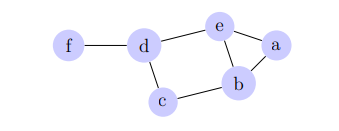
\includegraphics[width=0.5\linewidth]{Screenshot from 2024-12-03 11-29-17.png}
    \caption{}
    \label{fig:Problem 3}
\end{figure}

(a) (16 points) Prove that \textbf{LONG-PATH} is NP-Hard by reduction from one of the following: 3-SAT, CLIQUE, INDEPENDENT SET, VERTEX COVER, 3-COLORABLE, or HAMILTONIAN-CYCLE.\\


To prove that this is NP, we need to show that it can be tested in P-time. Given a long path, use BFS to traverse the path and count the number of edges and vertices to prove if True or False. This can be accomplished in O(n) time.




\section{11/26}
2-Clique: Given a graph $G$, determine if there's a 2-clique (i.e. an edge) in the graph.
This is in P because you can determine if there is an edge in linear time.

3-Clique: Given a graph $G$, determine if there's a 3-clique (i.e. a triangle) in the graph.
This is in P because in $n^3$ time you can consider all possible triples of vertices and see if any of them are a triangle.

$n-1$-Clique: Loop over all vertices, $v$ in the graph.  Consider the graph $V-v$, check to see if that graph is a clique (takes $n^2$ time).  If this is true for any $v$ then there is a $n-1$.  Takes polynomial time.

$n/2$-Clique: Given a graph $G$, determine if there's a $n/2$ clique in the graph.

In the reduction from 3-SAT to CLIQUE, we showed that $n/3$-CLIQUE is NP-HARD.


\section{11/19}
Recursion Cat with nodes that have real number values.  
A path is \emph{valid} if at any step of the path, the sum of the weights on all nodes is non-negative.

The cat starts at the root of a tree and wants to find if there is a valid to a node $v$.

Part (a):  Use dynamic programming to solve this.

For a node $v$, let $f(v)$ equal the sum of weights on all nodes on the path from the root node to the node $v$ if there is a valid path and $-\infty$ otherwise.

For a node $v$, let $w(v)$ be the weight of $v$.
Write a recurrence relation for the value of $f(v)$.  Let r be the root node. Let $p(v)$ be the parent of the node $v$.

Let $r$ be the root node
\[
f(r) = 
\begin{cases}
    w(r) & \text{if $w(r) \geq 0$}\\
    -\infty
\end{cases}\\
\]
Otherwise if $v \neq r$:
\[
f(v)=
    \begin{cases}
        -\infty & \text{if $f(p(v)) + w(v) < 0$}\\
        $f(p(v))+w(v)$ & \text{o.w.}
    \end{cases}
\]





\section{11/14}

\subsection{Problem of the Day}
A \emph{Clique} is a graph where every pair of node in the graph has an edge between them.

\begin{fact}
Any clique over $n$ nodes has ${n \choose 2} = \frac{n(n-1)}{2}$ edges.
\end{fact}

\begin{proof}
    \section*{Base Case}
    for n = 1 nodes there a 0 edges it is a clique and $n(n-1)/2 = 0$.
    \section*{Inductive Hypothesis}
    let us assume that for a clique having j nodes $\forall 1 \leq j < n $ has ((j-1)*(j-2))/2 edges 
    \section*{Inductive Step}
    Consider a clique, $G$ of $n$ nodes.  Remove some node $v$ in $G$ and the $n-1$ edges incident to $v$ to get a clique $G'$ over $n-1$ nodes.  By the IH, $G'$ has $(n-1)(n-2)/2$ edges.\\\\
    therefore total no of edges in the clique of n nodes is : (n-1)(n-2)/2 + (n-1) \\\\
    = (n-1)(n-2+2)/2 = n(n-1)/2 \\\\
\end{proof}



\subsection{WRONG!: Buildup "Proof" by Induction}

THIS IS WRONG!!!  In particular the ``fact" doesn't hold if you have two cycles of length $3$.
\begin{fact}
    Any graph where every node has degree at least $1$ is connected.
\end{fact}

WRONG!!
\begin{proof}
    Attempt by ``Build UP"
    We will show this by induction on $n$.\\
\noindent
    BC: $n = 1$, a single node graph is connected, since the single node can reach itself with the ``empty" path.\\
\noindent
IH: Any graph with $n$ nodes where every node has degree $1$ is connected.\\
\noindent
IS: Now start with a graph with $n$ nodes and a node $v$ to it.  By assumption this added node has degree at least $1$.  By the IH, the graph with $n$ nodes is connected.  Thus, since the node $v$ has degree at least $1$, it must be connected to the graph with $n$ nodes, and so this new graph with $n+1$ nodes is connected.   QED.
\end{proof}

Why does this go wrong?  Because you weren't able to build up to an \emph{arbitrary} graph.  This is why the ``build up" approach almost always fails when you're trying to do induction over graphs.  It is not trustworthy.  Do not use it! 

Instead use the correct approach that I've been teaching where you start with an arbitrary graph and make it smaller!





\section{11/12}
Induction problem over graphs.\\

A \emph{proper coloring} of a graph $G = (V,E)$ is an assignment of a color to each node in $V$ such that $\forall (u,v) \in E$, node $u$ and $v$ have different colors.

A \emph{$k$-coloring} of a graph $G = (V,E)$ is a proper coloring of $G$ that uses at most $k$ colors.

The problem of the day:

Prove that any graph $G = (V,E)$ with maximum degree $d$ can be colored with at most $d+1$ colors.

Idea: Do induction on the number of nodes in $G$, $n$.

\noindent
\textbf{BC: $n = 1$} Can color with $1$ color, which is no more than $d+1$.

\noindent
\textbf{IH:} Any graph with less than $n$ nodes and maximum degree $d$ can be colored with $d+1$ colors.

\noindent
\textbf{IS:} Consider a graph $G = (V,E)$ with $n$ nodes and maximum degree $d$.  Consider any node $v \in V$ and let $G'$ be graph with $v$ and all of its incident edges removed.  Since $G'$ has less than $n$ nodes, we can apply IH to say that $G'$ can be colored with $d+1$ colors.  We can color $v$ with a color that is missing from the no more than $d$ neighbors of $v$.  This gives a $d+1$ coloring of $G$.



If there is at least on node with degree zero there is one color that is needed to color the graph. 0+1 =1\\

Hint: Try induction over the number of nodes in $V$, not on the max degree!  
I.e.  IH: For any graph with $j<n$ nodes, .... [you fill in this]


Idea: do induction on $d$
BC $d = 0$

\textbf{IH:}
for all $j<d$; any graph $G=(V,E)$ with max degree $j$ can be colored with at most $j+1$ colors.

\textbf{IS:}
Consider a graph with maximum degree $d$.  


Let us have a graph $G$ with degree $n$, and now we reduce to $n-1$.



\section{10/28}
Race Track Problem: 

You are given a set of $n$ nodes connected in a cycle.  Each node has a non-negative weight, giving the gas at that node, each edge has a negative weight giving the amount of gas needed to traverse that edge.

The sum of the gas at all the nodes is at least equal to the negative of the sum of the weights on all edges.

You have a car with an infinite capacity gas tank.  Prove by induction that there is a location on the cycle that you can start from to complete a clockwise tour of the entire cycle without running out of gas.


\textbf{Claim:}That there exists a node such that we will not run out of gas from 1 tour of the cycle. 
\begin{proof}
By induction on $n$, the number of nodes in the cycle.    

\textbf{B.C.}n = 1\\
By the problem definition there will be a positive weight assigned to the node. Thus it is true that for a cost of zero any positive number will be greater than the zero. 

\textbf{I.H.}\\ $\forall 0<j<n$; If there's a cycle where the sum of gas at least equals sum of edge costs then there is a starting point to complete the cycle.  
\textbf{I.S.}\\
Consider a cycle, $C$ with $n$ nodes.  We will find a node edge pair $(v,e)$ where the gas available at the node at least equals the gas needed at the edge.  We can prove by contradiction that such a pair exists, because otherwise, the sum of gas on all nodes would be less than the sum of gas needed at all edges.

We create a new cycle $C'$ with $n-1$ nodes, by removing the pair $(v,e)$ and adding gas value of $w(v) - w(e)$ to the node that the edge points to, $w$.  Note that $C'$ has sum of gas available at least equal to sum of gas needed.  So, by the IH, there must be some node, $s$, in $C'$ we can start at and complete a tour of $C'$.  If $s \neq v$, then we can start at node $s$ for a correct tour of $C$.  If $s = w$, then we can start at node $v$ for a correct tour of $C$. 
In both cases the gas available at the deleted node, edge pair $(v,e)$ will allow us to traverse $e$ so we get a correct tour.

\end{proof}



\section{9/26}

$f(i) = 1/3 f(i-1) + 1/6 f(i-2)$
$f_i = f(i)$

Let $f = \langle f_1, f_2, \ldots \rangle = \langle f_i \rangle$.

Then 
$$f = \langle f_i \rangle$$
$$Lf = \langle f_{i+1} \rangle$$
$$L^2f = \langle f_{i+2} \rangle = \langle (1/3) f_{i+1} + (1/6) f_i \rangle$$

So,

$$L^2f - (1/3) Lf - (1/6) f = \langle 0 \rangle.$$

Thus the annihilator is 
$L^2 - (1/3)L - 1/6$


\section{9/17}

\subsection{Problem 1}

\subsubsection{Part (a)}
We have that $af(x/b) \geq K f(x)$ for all $x$, for fixed $K > 1$.
Problem 1, induction on $i$.
\begin{fact}
    $a^{i} f(n/b^{i}) \geq K^i f(n)$, for $i \in [0,\ell]$
\end{fact}


\begin{proof}
Proof is by induction on $i$.
    BC: $i = 0$, true since $a^0 = b^0 = K^0 = 1$ and so $a^0f(n/b^0) \geq K^0 f(n)$.\\
    IH: For all $0 \leq j<i$, $a^jf(n/b^j) \geq K^j f(n)$\\
    IS: 
    \begin{align*}
        a^{i} f(n/b^{i}) & = a^{i-1} a f(n/b^{i})\\
        & \geq K (a^{i-1} f(n/b^{i-1})) & \text{Since if $x \leftarrow n/b^{i-1}$, then $a f(n/b^i) \geq K f(n/b^{i-1})$}\\
        & \geq K (K^{i-1} f(n)) & \text{By the IH}\\
        & \geq K^i f(n)).
    \end{align*}
\end{proof}

\subsubsection{Part (b)}
We want to get an upperbound on $a^{\ell -j} f(n/b^{\ell -j})$ for $j$ going from $j = 0 \ldots \ell$ 
We've proven from part (a) that, for $i \in [1,\ell]$:
$$a^{i} f(n/b^{i}) \geq K^i f(x)$$

What happens if we set $x \leftarrow n/b^{\ell - j}$ and set $i$ so that $n/b^{i+\ell -j} = n/b^{\ell}$?  So $i \leftarrow j$.  Then we get:
$$a^{j} f(n/b^{\ell}) \geq K^j f(n/b^{\ell-j})$$

Now, multiplying both sides by $a^{\ell-j}$, we get:
$$a^{\ell} f(n/b^{\ell}) \geq K^j a^{\ell-j} f(n/b^{\ell-j})$$
Multiply both sides by $(1/K)^j$ we get:
$$\left(\frac{1}{K} \right)^j a^{\ell} f(n/b^{\ell}) \geq a^{\ell-j} f(n/b^{\ell-j})$$
letting $K' = 1/K$, note that $K'<1$.
$$(K')^j a^{\ell} f(n/b^{\ell}) \geq a^{\ell-j} f(n/b^{\ell-j})$$


\subsection{Knights and Knaves}
Let $f(n)$ be the maximum number of questions asked by our algorithm (discussed orally in section)
Recurrence relation is like
$$f(n) = f(n/2) + 2n$$

Root node is: $2n$; the second level is $n$ so there is a geometric decrease so the root node dominates.  So $f(n) = \Theta(n)$.


\section{9/12}
Problem 7-3 
\textbf{Part (a)}
The pivot is chosen uniformly at random from all $n$ elements.  So for a fixed element, the number of ways that element can be chosen is $1$ out of $n$ possible outcomes for the pivot.  So the probability $1/n$.  Let $X_i$ be $1$ if $i$-th smallest element chosen and $0$ otherwise.  Then $E(X_i) = 1 (1/n)$.

\textbf{Part (b)}
Let $T(n)$ be a r.v. giving the run time of quicksort on an array of size $n$.  Show that
    $$E(T(n)) = E\left(\sum_{q=1}^n X_q \left(T(q-1) + T(n-q) + \Theta(n) \right) \right)$$
The above holds, since there is exactly one element, call it the $r$-the smallest chosen as the pivot.  The value $X_r$ then equals $1$ and the expected runtime of the randomized quicksort is then given as

$$E(\left(T(r-1) + T(r-q) + \Theta(n) \right)$$
where $\Theta(n)$ is the cost for the partition and $T(r-1)$ is the cost of the recursive call on left side, $T(r-q)$ is the cost of the recursive call on the right side. (Note that $T(r-1)$ and $T(r-q)$ are random variables.).  

In the sum, $X_r = 1$ so one of the summands will be the above: $$E(\left(T(r-1) + T(r-q) + \Theta(n) \right)$$  Also, that for all $q \neq r$, $X_q = 0$ so there are no other summands


\textbf{Part (c)}

By part(a) for any $i$ $E(X_i)=1/n$.  So by linearity of expectation:
\begin{align*}
        E(T(n)) & = \sum_{q=1}^n E(X_q) E\left(\left(T(q-1) + T(n-q) + \Theta(n) \right) \right)\\
        & = \sum_{q=1}^n (1/n) E\left(\left(T(q-1) + T(n-q) + \Theta(n) \right) \right)\\
\end{align*}

    
\begin{align*}
    (1/n) \sum_{q=1}^n E\left(\left(T(q-1) + T(n-q) + \Theta(n) \right) \right) & = E(T(0)) + E(T(n-1)) + E(T(1)) + E(T(n-2)) + E(T(2)) + E(T(n-3)) + E(T(3)) + E(T(n-4)) + \ldots E(T(n-2)) + E(T(1)) + E(T(n-1)) + E(T(0)) + n \Theta(n)\\
    & = (2/n) \sum_{q=0}^{n-1} E\left(\left(T(q)) + \Theta(n) \right) \right)
\end{align*}

\medskip
\textbf{Part (d)}

\begin{align*}
    \sum_{k=2}^{n-1} k \log k & = \sum_{k=2}^{n/2} k \log (n/2) + \sum_{k=n/2 + 1}^{n-1} k \log n\\
    & = \sum_{k=2}^{n/2} k (\log n - 1) + \sum_{k=n/2 + 1}^{n-1} k \log n\\
    & = \sum_{k=2}^{n/2} k \log n  - \sum_{k=2}^{n/2} k  + \sum_{k=n/2 + 1}^{n-1} k \log n\\
    & = \sum_{k=2}^{n-1} k \log n  - \sum_{k=2}^{n/2} k\\
    & = \log n \sum_{k=2}^{n-1} k  - \sum_{k=2}^{n/2} k\\
     & = \frac{(n-1)((n-1)+1)}{2} \log n - \frac{(n/2+1)((n/2))}{2}\\
    & = (1/2) n^2 \log n  - (1/8)n^2 & \text{after some algebra}\\
\end{align*}

\medskip
\textbf{Part (e)}
Proof by induction where the guess is that $E(T(n) \leq a n \log n$.

BC: $n=2$, $E(T(n) = c \leq a 2 \log 2$ for some constant $a$.

IH: For all $2 \leq j<n$, $E(T(j) \leq a j \log j$

IS:

\begin{align*}
    E(T(n))  & = (2/n) \sum_{q=0}^{n-1} E((T(q)) + \Theta(n)  \\
& = (2/n) \sum_{q=2}^{n-1} a q \log q + \Theta(n)\\
& = \frac{2}{n} \left(a ((1/2) n^2 \log n  - (1/8)n^2) + \Theta(n^2) \right)\\
& \leq a n \log n \\
\end{align*}
Second step holds by the IH.  Third step holds by part (d)

The last step holds for $a$ sufficiently large (so that $ a(1/8)n^2) \geq$ the $\Theta(n^2))$ term.

\section{9/10, Phone drop problem}
Let $T(x,k)$ be the maximum number of drops needed if we have $x$ rungs and $k=3$ phones
\begin{align*}
    T(n,3) & = n/x + T(x,2)\\
           & = n/x + 2 \sqrt{x}\\
\end{align*}

To minimize this, see below to get that it is minimized when $x = n^{2/3}$.

\subsection{Calculus interlude}
To minimize this function of x, we can set $f(x) = n/x + 2x^{1/2}$ and find the minimum of this by taking the derivative with respect to $x$.  We get $f'(x) = -n x^{-2} + x^{-1/2}$.  Setting this equal to $0$, we get that $-nx^{-2} = - x^{-1/2}$.   This gives $nx^{-3/2} = 1$ or $n = x^{3/2}$ or $x = n^{2/3}$

\subsection{Back to the problem}

If we simplify and plug in $x = n^{2/3}$, we get:

\begin{align*}
    T(n,3) & = n/x + 2 \sqrt{x}\\
    & = n^{1/3} + 2 (n^{1/3})\\
    & = 3n^{1/3}
\end{align*}

$T(n,1) = n$, $T(n,2) = 2 n^{1/2}$, $T(n,3) = 3 n^{1/3}$.  So let's try to show for any $k$, that we can get $T(n,k) \leq k n^{1/k}$.

\subsection{General $k$}
The algorithm for $k=1$ phone is to drop the phone on each rung moving from bottom to top.

The algorithm for $k>1$ phones: drop the first phone every $x = n^{(k-1)/k}$ and then recurse on the remaining $k-1$ phones and $x = n^{(k-1)/k}$ rungs that need to be checked.

The number of drops for the above algorithm is given by the recurrence relation:

$T(n,k) = n/x + T(x, k-1)$.  Plugging in $x = n^{(k-1)/k}$, we get 

$T(n,k) = n^{1/k} + T(x, k-1)$.  We prove by induction on $k$ that the solution to this recurrence relation is $T(n,k) \leq k n^{1/k}$.

\begin{fact}
    $T(n,k) \leq k n^{1/k}$
\end{fact}
\begin{proof}
    We prove this by induction on $k$.
    BC: $k=1$, we shown that $T(n,1) = n \leq 1\cdot n$.
    IH: For all $j<k$ and for all values of $x$, $T(x,j) \leq j x^{1/j}$.
    IS: 
\begin{align*}
    T(n,k) & = n^{1/k} + T(n^{(k-1)/k},k-1) & \text{by the above definition of the recurrence}\\
           & = n^{1/k} + (k-1) (n^{(k-1)/k})^{1/(k-1)} \\
           & n^{1/k} + (k-1) n^{1/k} \\
           & k n^{1/k}
\end{align*}
\end{proof}


\section{Online Lecture}

\begin{align*}
    \sum_{i=1}^{n-1} \sum_{j=i+1}^n E(X_{i,j}) & = \sum_{i=1}^{n-1} \sum_{j=i+1}^n \frac{2}{j-i+1}\\
     & = \sum_{i=1}^{n-1}  (\frac{2}{2} + \frac{2}{3} + \ldots \frac{2}{n-i+1}) \\
    & = \sum_{i=1}^{n-1} 2 \sum_{k=1}^{n-i} \frac{1}{k+1} \\
    & \leq \sum_{i=1}^{n-1} 2 \sum_{k=1}^{n} \frac{1}{k} \\
    & \leq 2 \sum_{i=1}^{n-1} (1 + \ln n) & \text{Integral Upper bound}\\
    & \leq 2 (n-1) (1 + \ln n)\\
    & = 2 n + 2 n \ln n\\
    & = \Theta(n \ln n)\\
\end{align*}


\section{8/29}

\subsection{Student Questions}

$10 n = O(n)$ but $10 n \neq o(n)$.

The reason for this is because in $o$ notation, you need to inequality holds for any positive constant $c$ for $n_0$ sufficiently.

Let's show that $10 n \neq o(n)$.  

If this were true, then by the definition, we would have:
For any positive $c$, there exists a positive $n_0$ such that
$0 \leq 10 n < c n$ for all $n \geq n_0$.\\

For this to be true, we would need (dividing both sides of the above by $n$)
$$ 10 < c$$
But this doesn't meet the requirement of the definition that the inequality holds for any c for $n_0$ sufficiently large.

Let's show that $10 \sqrt{n} = o(n)$.  

If this were true, then by the definition, we would need:
For any positive $c$, there exists a positive $n_0$ such that
$0 \leq 10 \sqrt{n} < c n$ for all $n \geq n_0$.\\

For this to be true, we would need (dividing both sides of the above by $n$)
$$ \frac{10}{\sqrt{n}} < c$$
This does hold for any positive $c$ for $n_0$ sufficiently large.
$c\sqrt{n} > 10$, true if $\sqrt{n} > 10/c$ or $n > 100/c^2$.

\medskip

\begin{align*}
    \lim_{n \rightarrow \infty} \frac{10\sqrt{n}}{n} & = \lim_{n \rightarrow \infty} \frac{5}{\sqrt{n}}\\
    & = 0 
\end{align*}


How to simplify $$2^{(\log n)^2}?$$

\begin{align*}
    2^{(\log n)^2} & = 2^{(\log n)(\log n)}\\
    & = (2^{(\log n)})^{\log n} & \text{Since $(x^yz) = (x^y)^z$} \\
    & = n^{\log n} \\
\end{align*}

\subsection{Current Homework}
Let $X$ be the outcome of a $3$-sided die. $Pr(X = 1) = Pr(X = 2) = Pr(X=3) = 1/3$.

We know $$E(X) = \sum_{i=1}^3 i Pr(X = i) = 2$$

We know $$E(X^2) = \sum_{i=1}^3 i^2 Pr(X = i) = 1^1 (1/3) + 2^2 (1/3) + 3^2 (1/3) = 14/3$$.  Note that this does not equal $(E(X))^2 = 2^2 = 4$.

\subsection{Socks Problem}

Say you have $10$ pairs of socks, you put them in the dryer and $5$ of the socks randomly disappear.  What is the expected number of pairs of socks that remain? 

Let $X$ be a random variable that is the number of pairs of socks that remain.  We want $E(X)$.

For every pair of socks $i \in [1,10]$, let $X_i$ be $1$ if both socks in pair $i$ survive $0$ otherwise.  Then,
$$X = \sum_{i=1}^5 X_i$$

What is $E(X_i) = 1 Pr(X_i = 1) + 0 Pr(X_i =0) = Pr(X_i = 1)$.

$Pr(X_i = 1)$ is the probability that neither sock in the pair is removed $\frac{{18 \choose 5}}{{20 \choose 5}} = 21/38$

\begin{align*}
    E(X) &= E(\sum_{i=1}^10 X_i)\\
         & = \sum_{i=1}^10 E(X_i) & \text{By LOE}\\
        & = 10 (21/38) 
\end{align*}


\section{8/27}

\subsection{Recitation Exercises}
Exercise 1:

Prove that $10 \log n = o(\log^2 n)$. \\

Must show:  For any positive $c$, there exists a positive $n_0$ such that
$0 \leq 10 \log n < c \log^2 n$ for all $n \geq n_0$.\\

Since $\log n > 0$ for $n > 1$, the inequality $0 \leq 10 \log n < c \log^2 n$ holds iff
$\frac{10 \log n}{(\log n)^{2}} < c \frac{(\log n)^{2}}{(\log n)^{2}}$\\
This holds iff:
$$\frac{10}{\log n} < c$$
By cross-multiplying, the above holds if $10 < c \log n$ or $\log n > 10/c$.  By raising both sides to the power of $2$ we get that this holds iff:
$2^{\log n} > 2^{10/c}$ or $n > 2^{10/c}$.

So $n_0 = 2^{10/c} + 1$

Exercise 2:
Prove that $2^n = o(3^n)$.

Must show:  For any positive $c$, there exists a positive $n_0$ such that
$0 \leq 2^n < c 3^n$ for all $n \geq n_0$.\\
For $n \geq 0$, the inequality is preserved if we take the log of both sides to get:

$$ n < \log c + n \log 3  $$
iff
$$ - \log c < n( \log 3 -1) $$

$$ - \frac{\log c}{\log 3} < n $$

So if we set $n_0 = (- \frac{\log c}{\log 3}) + 1$

(Note that $- \log c = \log 1/c$ since $\log c^{-1} = - \log c$.)

\medskip

\subsection{HW: $n! = o(n^n)$}

\medskip

Recall that $\log (xy) = \log x + \log y$.  Note that $n! = n (n-1) (n-2) \ldots 2 1 = \prod_{i=1}^n i$.

\begin{align*}
    \log n! & = \log n + \log (n-1) + \log (n-2) + \ldots \log 2 + \log 1 \\
    & \leq \log n + \log n + \log n + \ldots + \log n\\
    & = n \log n
\end{align*}

\begin{align*}
    \log n! & = \log n + \log (n-1) + \log (n-2) + \ldots \log 2 + \log 1 \\
    & \geq \log n/2 + \log n/2 + \ldots \log n/2 \\
\end{align*}

\section{8/22}
Problem:

Let $\displaystyle f( 1) \ =\ 1$, $\displaystyle f( 2) \ =\ 1$, for $\displaystyle n\geq 2$, $\displaystyle f( n) \ =\ f( n-1) \ +\ f( n-2)$.

$\displaystyle f( 3) \ =\ f( 2) \ +\ f( 1) \ =\ 2$, $\displaystyle f( 4) \ =\ f( 3) \ +\ f( 2) \ =\ 3$, $\displaystyle f( 5) \ =\ 5$, $\displaystyle f( 6) \ =\ 8$.	

\medskip

To prove: (1) $f(n) O\left( 2^{n}\right)$; and (2) $f(n) \Omega \left(( 3/2)^{n}\right)$

\medskip

\begin{fact}
    $\displaystyle f( n) \ =\ O\left( 2^{n}\right)$
\end{fact}

\begin{proof}
    Let $c$ be some constant to be determined.\\
BC: n = 1, $f(1) = 1 leq c2^1$ for $c \leq 1$

IH: For all $1 \leq j < n$, $f(j) \leq c2^{j}$ 

IS: 
\begin{align*}
    f(n) &= f(n-1) + f(n-2) \\
    & = c2^{n-1} + c2^{n-2} & \text{by IH}\\
    & \leq c2^{n-1} + c2^{n-1} \\
    & = c2^n
\end{align*}
The last step holds for $c = 1$.
\end{proof}

\newpage

\begin{fact}
    $f(n) = \Omega((3/2)^n)$
\end{fact}

\begin{proof}
    We must show that there exist positive constants $c$ and $n_0$ such that $0 \leq f(n) \geq c (3/2)^n$ for all $n \geq n_0$.

BC: $f(1) = 1 \geq c (3/2)^1$.  This is true for $c \leq 2/3$.

IH: For all $1 \leq j < n$, $f(j) \geq c (3/2)^j$.

IS: 
   \begin{align*}
    f(n) &= f(n-1) + f(n-2)\\
         &\geq c ((3/2)^{n-1} + (3/2)^{n-2}) & \text{by IH}\\
         & \geq c ((3/2)^{n-2}(3/2 + 1)\\
        & \geq c (5/2) ((3/2)^{n-2})\\
        & \geq c (5/2)(2/3)^2 ((3/2)^n)\\
        & \geq c ((3/2)^n)
\end{align*}
\end{proof}

\end{document}
